\documentclass[a4paper, 12pt]{article}
\usepackage[top=1.5cm, bottom=2.2cm, left=2cm, right=2cm]{geometry}
\usepackage[utf8]{inputenc}
\usepackage{graphicx, caption}
\usepackage{float}
\usepackage{amsmath, amsfonts, amssymb, esint}
\usepackage{hyperref}
\usepackage{multicol}
\usepackage{color}
\usepackage{wallpaper}
\usepackage{array}

\CenterWallPaper{1}{./img/background.png}

\hypersetup{
    colorlinks=true,
    linkcolor=blue,
    filecolor=magenta,      
    urlcolor=cyan,
}

\newcolumntype{M}[1]{>{\centering\arraybackslash}m{#1}}

\definecolor{red}{rgb}{1,0,0}
\newcommand{\red}[1]{\textcolor{red}{#1}}

\begin{document}
    \begin{figure}
        \centering
        \href{https://ligaolimpicadeastronomia.com.br/}{\includegraphics[scale=0.6]{./img/logos.png}}
    \end{figure}
    \begin{center}
        \begin{large}
            \textbf{Simulado 2 -- Intensivão para a OBA}
            \linebreak \red{Gabarito}
        \end{large}
        \end{center}
    \begin{flushright}
        Material elaborado por \textbf{Giulia Nóbrega} e \textbf{Iago Mendes}.
    \end{flushright}
    \red{Observação: \begin{itemize}
        \item As alternativas das perguntas deste gabarito não estão na mesma ordem do simulado.
    \end{itemize}}

    \section*{Questões de Astronomia}
        \begin{flushleft} \begin{itemize}
            \item \textbf{Questão 1) (1 ponto)} A imagem abaixo traz 2 constelações muito famosas. A partir da imagem, responda o que se pede:
                \begin{figure}[H]
                    \centering
                    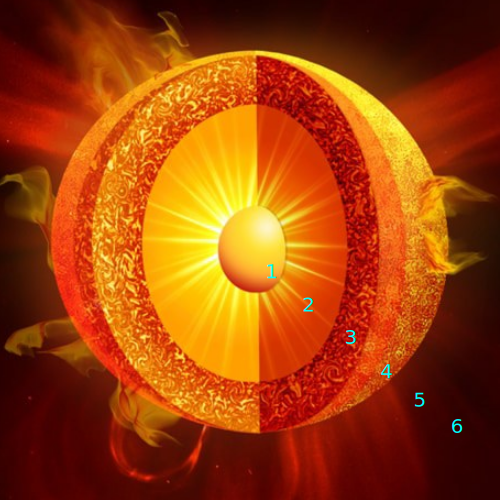
\includegraphics[scale=0.5]{./img/1.png}
                \end{figure}
                \begin{itemize}
                    \item \textbf{Pergunta 1a) (1 ponto) (0,5 ponto cada acerto)} Identifique quais são as constelações na imagem.
                    \begin{center} \begin{tabular}
                    {
                        |M{0.20\textwidth}|M{0.10\textwidth}|M{0.10\textwidth}|M{0.10\textwidth}|M{0.10\textwidth}|
                    }
                        \hline
                        $\quad$ & Centauro & Cruzeiro do Sul & Cisne & Ursa Maior \\ \hline
                        Constelação da esquerda & $\quad$ & \red{X} & $\quad$ & $\quad$ \\ \hline
                        Constelação da direita & $\quad$ & $\quad$ & $\quad$ & \red{X} \\ \hline
                    \end{tabular} \end{center}
                \end{itemize}
            
            
        \end{itemize} \end{flushleft}
    \section*{Questões de Astronáutica}
    \section*{Questões avançadas}
\end{document}